\documentclass[twoside]{book}

% Packages required by doxygen
\usepackage{fixltx2e}
\usepackage{calc}
\usepackage{doxygen}
\usepackage[export]{adjustbox} % also loads graphicx
\usepackage{graphicx}
\usepackage[utf8]{inputenc}
\usepackage{makeidx}
\usepackage{multicol}
\usepackage{multirow}
\PassOptionsToPackage{warn}{textcomp}
\usepackage{textcomp}
\usepackage[nointegrals]{wasysym}
\usepackage[table]{xcolor}

% Font selection
\usepackage[T1]{fontenc}
\usepackage[scaled=.90]{helvet}
\usepackage{courier}
\usepackage{amssymb}
\usepackage{sectsty}
\renewcommand{\familydefault}{\sfdefault}
\allsectionsfont{%
  \fontseries{bc}\selectfont%
  \color{darkgray}%
}
\renewcommand{\DoxyLabelFont}{%
  \fontseries{bc}\selectfont%
  \color{darkgray}%
}
\newcommand{\+}{\discretionary{\mbox{\scriptsize$\hookleftarrow$}}{}{}}

% Page & text layout
\usepackage{geometry}
\geometry{%
  a4paper,%
  top=2.5cm,%
  bottom=2.5cm,%
  left=2.5cm,%
  right=2.5cm%
}
\tolerance=750
\hfuzz=15pt
\hbadness=750
\setlength{\emergencystretch}{15pt}
\setlength{\parindent}{0cm}
\setlength{\parskip}{3ex plus 2ex minus 2ex}
\makeatletter
\renewcommand{\paragraph}{%
  \@startsection{paragraph}{4}{0ex}{-1.0ex}{1.0ex}{%
    \normalfont\normalsize\bfseries\SS@parafont%
  }%
}
\renewcommand{\subparagraph}{%
  \@startsection{subparagraph}{5}{0ex}{-1.0ex}{1.0ex}{%
    \normalfont\normalsize\bfseries\SS@subparafont%
  }%
}
\makeatother

% Headers & footers
\usepackage{fancyhdr}
\pagestyle{fancyplain}
\fancyhead[LE]{\fancyplain{}{\bfseries\thepage}}
\fancyhead[CE]{\fancyplain{}{}}
\fancyhead[RE]{\fancyplain{}{\bfseries\leftmark}}
\fancyhead[LO]{\fancyplain{}{\bfseries\rightmark}}
\fancyhead[CO]{\fancyplain{}{}}
\fancyhead[RO]{\fancyplain{}{\bfseries\thepage}}
\fancyfoot[LE]{\fancyplain{}{}}
\fancyfoot[CE]{\fancyplain{}{}}
\fancyfoot[RE]{\fancyplain{}{\bfseries\scriptsize Generated by Doxygen }}
\fancyfoot[LO]{\fancyplain{}{\bfseries\scriptsize Generated by Doxygen }}
\fancyfoot[CO]{\fancyplain{}{}}
\fancyfoot[RO]{\fancyplain{}{}}
\renewcommand{\footrulewidth}{0.4pt}
\renewcommand{\chaptermark}[1]{%
  \markboth{#1}{}%
}
\renewcommand{\sectionmark}[1]{%
  \markright{\thesection\ #1}%
}

% Indices & bibliography
\usepackage{natbib}
\usepackage[titles]{tocloft}
\setcounter{tocdepth}{3}
\setcounter{secnumdepth}{5}
\makeindex

% Hyperlinks (required, but should be loaded last)
\usepackage{ifpdf}
\ifpdf
  \usepackage[pdftex,pagebackref=true]{hyperref}
\else
  \usepackage[ps2pdf,pagebackref=true]{hyperref}
\fi
\hypersetup{%
  colorlinks=true,%
  linkcolor=blue,%
  citecolor=blue,%
  unicode%
}

% Custom commands
\newcommand{\clearemptydoublepage}{%
  \newpage{\pagestyle{empty}\cleardoublepage}%
}

\usepackage{caption}
\captionsetup{labelsep=space,justification=centering,font={bf},singlelinecheck=off,skip=4pt,position=top}

%===== C O N T E N T S =====

\begin{document}

% Titlepage & ToC
\hypersetup{pageanchor=false,
             bookmarksnumbered=true,
             pdfencoding=unicode
            }
\pagenumbering{alph}
\begin{titlepage}
\vspace*{7cm}
\begin{center}%
{\Large res\+Ervation }\\
\vspace*{1cm}
{\large Generated by Doxygen 1.8.13}\\
\end{center}
\end{titlepage}
\clearemptydoublepage
\pagenumbering{roman}
\tableofcontents
\clearemptydoublepage
\pagenumbering{arabic}
\hypersetup{pageanchor=true}

%--- Begin generated contents ---
\chapter{Hierarchical Index}
\section{Class Hierarchy}
This inheritance list is sorted roughly, but not completely, alphabetically\+:\begin{DoxyCompactList}
\item mysqli\begin{DoxyCompactList}
\item \contentsline{section}{class\+Res}{\pageref{classclass_res}}{}
\end{DoxyCompactList}
\end{DoxyCompactList}

\chapter{Data Structure Index}
\section{Data Structures}
Here are the data structures with brief descriptions\+:\begin{DoxyCompactList}
\item\contentsline{section}{\hyperlink{classclass_res}{class\+Res} }{\pageref{classclass_res}}{}
\end{DoxyCompactList}

\chapter{File Index}
\section{File List}
Here is a list of all files with brief descriptions\+:\begin{DoxyCompactList}
\item\contentsline{section}{/\+Users/rory/\+Sites/\+Res\+Ervation/public\+\_\+html/\hyperlink{asset_list_8php}{asset\+List.\+php} }{\pageref{asset_list_8php}}{}
\item\contentsline{section}{/\+Users/rory/\+Sites/\+Res\+Ervation/public\+\_\+html/\hyperlink{config_8php}{config.\+php} }{\pageref{config_8php}}{}
\item\contentsline{section}{/\+Users/rory/\+Sites/\+Res\+Ervation/public\+\_\+html/\hyperlink{index_8php}{index.\+php} }{\pageref{index_8php}}{}
\item\contentsline{section}{/\+Users/rory/\+Sites/\+Res\+Ervation/public\+\_\+html/\hyperlink{process_booking_8php}{process\+Booking.\+php} }{\pageref{process_booking_8php}}{}
\item\contentsline{section}{/\+Users/rory/\+Sites/\+Res\+Ervation/public\+\_\+html/\hyperlink{res_find_8php}{res\+Find.\+php} }{\pageref{res_find_8php}}{}
\item\contentsline{section}{/\+Users/rory/\+Sites/\+Res\+Ervation/public\+\_\+html/\hyperlink{search_result_8php}{search\+Result.\+php} }{\pageref{search_result_8php}}{}
\item\contentsline{section}{/\+Users/rory/\+Sites/\+Res\+Ervation/public\+\_\+html/classes/\hyperlink{class_res_8php}{class\+Res.\+php} }{\pageref{class_res_8php}}{}
\end{DoxyCompactList}

\chapter{Data Structure Documentation}
\hypertarget{classclass_res}{}\section{class\+Res Class Reference}
\label{classclass_res}\index{class\+Res@{class\+Res}}
Inheritance diagram for class\+Res\+:\begin{figure}[H]
\begin{center}
\leavevmode
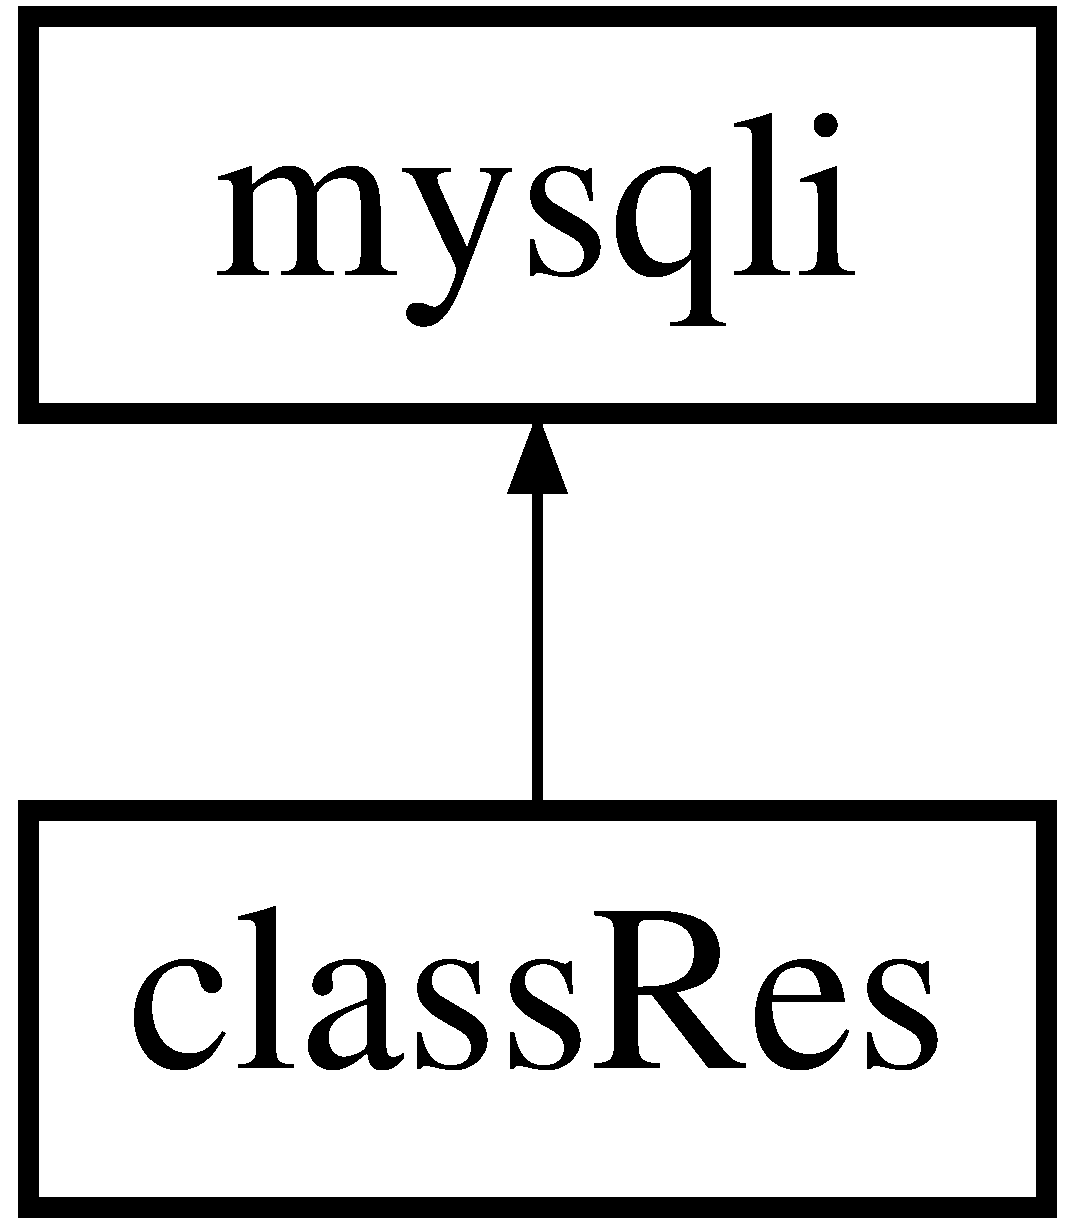
\includegraphics[height=2.000000cm]{classclass_res}
\end{center}
\end{figure}
\subsection*{Public Member Functions}
\begin{DoxyCompactItemize}
\item 
\hyperlink{classclass_res_a095c5d389db211932136b53f25f39685}{\+\_\+\+\_\+construct} ()
\item 
\hyperlink{classclass_res_ae8167da71e306192c7c2b3e4e9780383}{get\+Asset\+List} (\$start, \$end, \$duration, \$pax)
\item 
\hyperlink{classclass_res_a8556a92bb6f8fbbdb406cd29e6a6bf9f}{find\+Res} (\$search\+String)
\item 
\hyperlink{classclass_res_a5761febd4e36158c6513a63b9b862dd9}{get\+Next\+Res\+No} ()
\item 
\hyperlink{classclass_res_a6c5d3040d1db2b9d8000117b5b2539b7}{create\+Reservation} (\$info)
\end{DoxyCompactItemize}
\subsection*{Data Fields}
\begin{DoxyCompactItemize}
\item 
\hyperlink{classclass_res_a4d91186c9ddc5fdec9eddf319a4ab85e}{\$info\+Array}
\end{DoxyCompactItemize}


\subsection{Detailed Description}
Description of \hyperlink{classclass_res}{class\+Res}

\begin{DoxyAuthor}{Author}
rory
\end{DoxyAuthor}
\$info\+: ( \mbox{[}0\mbox{]} =$>$ std\+Class Object ( \mbox{[}id\mbox{]} =$>$ num\+Days \mbox{[}value\mbox{]} =$>$ ) ~\newline
 \mbox{[}1\mbox{]} =$>$ std\+Class Object ( \mbox{[}id\mbox{]} =$>$ start\+Day \mbox{[}value\mbox{]} =$>$ ) ~\newline
 \mbox{[}2\mbox{]} =$>$ std\+Class Object ( \mbox{[}id\mbox{]} =$>$ end\+Day \mbox{[}value\mbox{]} =$>$ ) ~\newline
 \mbox{[}3\mbox{]} =$>$ std\+Class Object ( \mbox{[}id\mbox{]} =$>$ Asset\+Id \mbox{[}value\mbox{]} =$>$ ) ~\newline
 \mbox{[}4\mbox{]} =$>$ std\+Class Object ( \mbox{[}id\mbox{]} =$>$ Tel \mbox{[}value\mbox{]} =$>$ ) ~\newline
 \mbox{[}5\mbox{]} =$>$ std\+Class Object ( \mbox{[}id\mbox{]} =$>$ F\+Name \mbox{[}value\mbox{]} =$>$ ) ~\newline
 \mbox{[}6\mbox{]} =$>$ std\+Class Object ( \mbox{[}id\mbox{]} =$>$ S\+Name \mbox{[}value\mbox{]} =$>$ ) ~\newline
 \mbox{[}7\mbox{]} =$>$ std\+Class Object ( \mbox{[}id\mbox{]} =$>$ email \mbox{[}value\mbox{]} =$>$ ))~\newline
 ~\newline
 reservations stored nightly -\/ each night has own record with common Reservation Number~\newline
 

Definition at line 20 of file class\+Res.\+php.



\subsection{Constructor \& Destructor Documentation}
\mbox{\Hypertarget{classclass_res_a095c5d389db211932136b53f25f39685}\label{classclass_res_a095c5d389db211932136b53f25f39685}} 
\index{class\+Res@{class\+Res}!\+\_\+\+\_\+construct@{\+\_\+\+\_\+construct}}
\index{\+\_\+\+\_\+construct@{\+\_\+\+\_\+construct}!class\+Res@{class\+Res}}
\subsubsection{\texorpdfstring{\+\_\+\+\_\+construct()}{\_\_construct()}}
{\footnotesize\ttfamily \+\_\+\+\_\+construct (\begin{DoxyParamCaption}{ }\end{DoxyParamCaption})}



Definition at line 26 of file class\+Res.\+php.



\subsection{Member Function Documentation}
\mbox{\Hypertarget{classclass_res_a6c5d3040d1db2b9d8000117b5b2539b7}\label{classclass_res_a6c5d3040d1db2b9d8000117b5b2539b7}} 
\index{class\+Res@{class\+Res}!create\+Reservation@{create\+Reservation}}
\index{create\+Reservation@{create\+Reservation}!class\+Res@{class\+Res}}
\subsubsection{\texorpdfstring{create\+Reservation()}{createReservation()}}
{\footnotesize\ttfamily create\+Reservation (\begin{DoxyParamCaption}\item[{}]{\$info }\end{DoxyParamCaption})}



Definition at line 79 of file class\+Res.\+php.

\mbox{\Hypertarget{classclass_res_a8556a92bb6f8fbbdb406cd29e6a6bf9f}\label{classclass_res_a8556a92bb6f8fbbdb406cd29e6a6bf9f}} 
\index{class\+Res@{class\+Res}!find\+Res@{find\+Res}}
\index{find\+Res@{find\+Res}!class\+Res@{class\+Res}}
\subsubsection{\texorpdfstring{find\+Res()}{findRes()}}
{\footnotesize\ttfamily find\+Res (\begin{DoxyParamCaption}\item[{}]{\$search\+String }\end{DoxyParamCaption})}



Definition at line 44 of file class\+Res.\+php.

\mbox{\Hypertarget{classclass_res_ae8167da71e306192c7c2b3e4e9780383}\label{classclass_res_ae8167da71e306192c7c2b3e4e9780383}} 
\index{class\+Res@{class\+Res}!get\+Asset\+List@{get\+Asset\+List}}
\index{get\+Asset\+List@{get\+Asset\+List}!class\+Res@{class\+Res}}
\subsubsection{\texorpdfstring{get\+Asset\+List()}{getAssetList()}}
{\footnotesize\ttfamily get\+Asset\+List (\begin{DoxyParamCaption}\item[{}]{\$start,  }\item[{}]{\$end,  }\item[{}]{\$duration,  }\item[{}]{\$pax }\end{DoxyParamCaption})}



Definition at line 31 of file class\+Res.\+php.

\mbox{\Hypertarget{classclass_res_a5761febd4e36158c6513a63b9b862dd9}\label{classclass_res_a5761febd4e36158c6513a63b9b862dd9}} 
\index{class\+Res@{class\+Res}!get\+Next\+Res\+No@{get\+Next\+Res\+No}}
\index{get\+Next\+Res\+No@{get\+Next\+Res\+No}!class\+Res@{class\+Res}}
\subsubsection{\texorpdfstring{get\+Next\+Res\+No()}{getNextResNo()}}
{\footnotesize\ttfamily get\+Next\+Res\+No (\begin{DoxyParamCaption}{ }\end{DoxyParamCaption})}



Definition at line 74 of file class\+Res.\+php.



\subsection{Field Documentation}
\mbox{\Hypertarget{classclass_res_a4d91186c9ddc5fdec9eddf319a4ab85e}\label{classclass_res_a4d91186c9ddc5fdec9eddf319a4ab85e}} 
\index{class\+Res@{class\+Res}!\$info\+Array@{\$info\+Array}}
\index{\$info\+Array@{\$info\+Array}!class\+Res@{class\+Res}}
\subsubsection{\texorpdfstring{\$info\+Array}{$infoArray}}
{\footnotesize\ttfamily \$info\+Array}



Definition at line 24 of file class\+Res.\+php.



The documentation for this class was generated from the following file\+:\begin{DoxyCompactItemize}
\item 
/\+Users/rory/\+Sites/\+Res\+Ervation/public\+\_\+html/classes/\hyperlink{class_res_8php}{class\+Res.\+php}\end{DoxyCompactItemize}

\chapter{File Documentation}
\hypertarget{asset_list_8php}{}\section{/\+Users/rory/\+Sites/\+Res\+Ervation/public\+\_\+html/asset\+List.php File Reference}
\label{asset_list_8php}\index{/\+Users/rory/\+Sites/\+Res\+Ervation/public\+\_\+html/asset\+List.\+php@{/\+Users/rory/\+Sites/\+Res\+Ervation/public\+\_\+html/asset\+List.\+php}}
\subsection*{Variables}
\begin{DoxyCompactItemize}
\item 
\hyperlink{asset_list_8php_a50a00e7de77365e00b117e73aa82fb9b}{\$start} = filter\+\_\+input(I\+N\+P\+U\+T\+\_\+\+G\+ET, \textquotesingle{}start\textquotesingle{})
\item 
\hyperlink{asset_list_8php_ac2040b96cd66d4d79b1d9fe0027d2f9b}{\$end} = filter\+\_\+input(I\+N\+P\+U\+T\+\_\+\+G\+ET, \textquotesingle{}end\textquotesingle{})
\item 
\hyperlink{asset_list_8php_acae43950182b63cd06434397298dad7d}{\$duration} = filter\+\_\+input(I\+N\+P\+U\+T\+\_\+\+G\+ET, \textquotesingle{}duration\textquotesingle{})
\item 
\hyperlink{asset_list_8php_aa1164ec0ca5257a40108859a07302f7b}{\$pax} = filter\+\_\+input(I\+N\+P\+U\+T\+\_\+\+G\+ET, \textquotesingle{}pax\textquotesingle{})
\item 
\hyperlink{asset_list_8php_a1646d1b5d10f701de3a7c119f7fe1013}{\$\+Res} = new class\+Res()
\item 
\hyperlink{asset_list_8php_a51f80498ef842363e219cfadcf05128e}{\$\+Asset\+List} = \$Res-\/$>$get\+Asset\+List(\$start, \$end, \$duration, \$pax)
\end{DoxyCompactItemize}


\subsection{Variable Documentation}
\mbox{\Hypertarget{asset_list_8php_a51f80498ef842363e219cfadcf05128e}\label{asset_list_8php_a51f80498ef842363e219cfadcf05128e}} 
\index{asset\+List.\+php@{asset\+List.\+php}!\$\+Asset\+List@{\$\+Asset\+List}}
\index{\$\+Asset\+List@{\$\+Asset\+List}!asset\+List.\+php@{asset\+List.\+php}}
\subsubsection{\texorpdfstring{\$\+Asset\+List}{$AssetList}}
{\footnotesize\ttfamily \$Asset\+List = \$Res-\/$>$get\+Asset\+List(\$start, \$end, \$duration, \$pax)}



Definition at line 11 of file asset\+List.\+php.

\mbox{\Hypertarget{asset_list_8php_acae43950182b63cd06434397298dad7d}\label{asset_list_8php_acae43950182b63cd06434397298dad7d}} 
\index{asset\+List.\+php@{asset\+List.\+php}!\$duration@{\$duration}}
\index{\$duration@{\$duration}!asset\+List.\+php@{asset\+List.\+php}}
\subsubsection{\texorpdfstring{\$duration}{$duration}}
{\footnotesize\ttfamily \$duration = filter\+\_\+input(I\+N\+P\+U\+T\+\_\+\+G\+ET, \textquotesingle{}duration\textquotesingle{})}



Definition at line 8 of file asset\+List.\+php.

\mbox{\Hypertarget{asset_list_8php_ac2040b96cd66d4d79b1d9fe0027d2f9b}\label{asset_list_8php_ac2040b96cd66d4d79b1d9fe0027d2f9b}} 
\index{asset\+List.\+php@{asset\+List.\+php}!\$end@{\$end}}
\index{\$end@{\$end}!asset\+List.\+php@{asset\+List.\+php}}
\subsubsection{\texorpdfstring{\$end}{$end}}
{\footnotesize\ttfamily \$end = filter\+\_\+input(I\+N\+P\+U\+T\+\_\+\+G\+ET, \textquotesingle{}end\textquotesingle{})}



Definition at line 7 of file asset\+List.\+php.

\mbox{\Hypertarget{asset_list_8php_aa1164ec0ca5257a40108859a07302f7b}\label{asset_list_8php_aa1164ec0ca5257a40108859a07302f7b}} 
\index{asset\+List.\+php@{asset\+List.\+php}!\$pax@{\$pax}}
\index{\$pax@{\$pax}!asset\+List.\+php@{asset\+List.\+php}}
\subsubsection{\texorpdfstring{\$pax}{$pax}}
{\footnotesize\ttfamily \$pax = filter\+\_\+input(I\+N\+P\+U\+T\+\_\+\+G\+ET, \textquotesingle{}pax\textquotesingle{})}



Definition at line 9 of file asset\+List.\+php.

\mbox{\Hypertarget{asset_list_8php_a1646d1b5d10f701de3a7c119f7fe1013}\label{asset_list_8php_a1646d1b5d10f701de3a7c119f7fe1013}} 
\index{asset\+List.\+php@{asset\+List.\+php}!\$\+Res@{\$\+Res}}
\index{\$\+Res@{\$\+Res}!asset\+List.\+php@{asset\+List.\+php}}
\subsubsection{\texorpdfstring{\$\+Res}{$Res}}
{\footnotesize\ttfamily \$Res = new class\+Res()}



Definition at line 10 of file asset\+List.\+php.

\mbox{\Hypertarget{asset_list_8php_a50a00e7de77365e00b117e73aa82fb9b}\label{asset_list_8php_a50a00e7de77365e00b117e73aa82fb9b}} 
\index{asset\+List.\+php@{asset\+List.\+php}!\$start@{\$start}}
\index{\$start@{\$start}!asset\+List.\+php@{asset\+List.\+php}}
\subsubsection{\texorpdfstring{\$start}{$start}}
{\footnotesize\ttfamily \$start = filter\+\_\+input(I\+N\+P\+U\+T\+\_\+\+G\+ET, \textquotesingle{}start\textquotesingle{})}



Definition at line 6 of file asset\+List.\+php.


\hypertarget{class_res_8php}{}\section{/\+Users/rory/\+Sites/\+Res\+Ervation/public\+\_\+html/classes/class\+Res.php File Reference}
\label{class_res_8php}\index{/\+Users/rory/\+Sites/\+Res\+Ervation/public\+\_\+html/classes/class\+Res.\+php@{/\+Users/rory/\+Sites/\+Res\+Ervation/public\+\_\+html/classes/class\+Res.\+php}}
\subsection*{Data Structures}
\begin{DoxyCompactItemize}
\item 
class \hyperlink{classclass_res}{class\+Res}
\end{DoxyCompactItemize}

\hypertarget{config_8php}{}\section{/\+Users/rory/\+Sites/\+Res\+Ervation/public\+\_\+html/config.php File Reference}
\label{config_8php}\index{/\+Users/rory/\+Sites/\+Res\+Ervation/public\+\_\+html/config.\+php@{/\+Users/rory/\+Sites/\+Res\+Ervation/public\+\_\+html/config.\+php}}
\subsection*{Variables}
\begin{DoxyCompactItemize}
\item 
const \hyperlink{config_8php_a293363d7988627f671958e2d908c202a}{D\+B\+\_\+\+H\+O\+ST} \textquotesingle{}localhost\textquotesingle{}
\item 
const \hyperlink{config_8php_ab5db0d3504f917f268614c50b02c53e2}{D\+B\+\_\+\+N\+A\+ME} \textquotesingle{}res\+Ervation\textquotesingle{}
\item 
const \hyperlink{config_8php_a1d1d99f8e08f387d84fe9848f3357156}{D\+B\+\_\+\+U\+S\+ER} \textquotesingle{}res\+Web\+User\textquotesingle{}
\item 
const \hyperlink{config_8php_a8bb9c4546d91667cfa61879d83127a92}{D\+B\+\_\+\+P\+A\+SS} \textquotesingle{}Some\+Long\+Convoluted\+Password\textquotesingle{}
\item 
const \hyperlink{config_8php_a2e7ab70d786ad1c2e3c1f87f15b3df27}{T\+O\+D\+AY} gmdate(\char`\"{}Y-\/m-\/d H\+:i\+:s\char`\"{}, strtotime(\char`\"{} + 2 hours\char`\"{}))
\end{DoxyCompactItemize}


\subsection{Variable Documentation}
\mbox{\Hypertarget{config_8php_a293363d7988627f671958e2d908c202a}\label{config_8php_a293363d7988627f671958e2d908c202a}} 
\index{config.\+php@{config.\+php}!D\+B\+\_\+\+H\+O\+ST@{D\+B\+\_\+\+H\+O\+ST}}
\index{D\+B\+\_\+\+H\+O\+ST@{D\+B\+\_\+\+H\+O\+ST}!config.\+php@{config.\+php}}
\subsubsection{\texorpdfstring{D\+B\+\_\+\+H\+O\+ST}{DB\_HOST}}
{\footnotesize\ttfamily const D\+B\+\_\+\+H\+O\+ST \textquotesingle{}localhost\textquotesingle{}}



Definition at line 3 of file config.\+php.

\mbox{\Hypertarget{config_8php_ab5db0d3504f917f268614c50b02c53e2}\label{config_8php_ab5db0d3504f917f268614c50b02c53e2}} 
\index{config.\+php@{config.\+php}!D\+B\+\_\+\+N\+A\+ME@{D\+B\+\_\+\+N\+A\+ME}}
\index{D\+B\+\_\+\+N\+A\+ME@{D\+B\+\_\+\+N\+A\+ME}!config.\+php@{config.\+php}}
\subsubsection{\texorpdfstring{D\+B\+\_\+\+N\+A\+ME}{DB\_NAME}}
{\footnotesize\ttfamily const D\+B\+\_\+\+N\+A\+ME \textquotesingle{}res\+Ervation\textquotesingle{}}



Definition at line 4 of file config.\+php.

\mbox{\Hypertarget{config_8php_a8bb9c4546d91667cfa61879d83127a92}\label{config_8php_a8bb9c4546d91667cfa61879d83127a92}} 
\index{config.\+php@{config.\+php}!D\+B\+\_\+\+P\+A\+SS@{D\+B\+\_\+\+P\+A\+SS}}
\index{D\+B\+\_\+\+P\+A\+SS@{D\+B\+\_\+\+P\+A\+SS}!config.\+php@{config.\+php}}
\subsubsection{\texorpdfstring{D\+B\+\_\+\+P\+A\+SS}{DB\_PASS}}
{\footnotesize\ttfamily const D\+B\+\_\+\+P\+A\+SS \textquotesingle{}Some\+Long\+Convoluted\+Password\textquotesingle{}}



Definition at line 6 of file config.\+php.

\mbox{\Hypertarget{config_8php_a1d1d99f8e08f387d84fe9848f3357156}\label{config_8php_a1d1d99f8e08f387d84fe9848f3357156}} 
\index{config.\+php@{config.\+php}!D\+B\+\_\+\+U\+S\+ER@{D\+B\+\_\+\+U\+S\+ER}}
\index{D\+B\+\_\+\+U\+S\+ER@{D\+B\+\_\+\+U\+S\+ER}!config.\+php@{config.\+php}}
\subsubsection{\texorpdfstring{D\+B\+\_\+\+U\+S\+ER}{DB\_USER}}
{\footnotesize\ttfamily const D\+B\+\_\+\+U\+S\+ER \textquotesingle{}res\+Web\+User\textquotesingle{}}



Definition at line 5 of file config.\+php.

\mbox{\Hypertarget{config_8php_a2e7ab70d786ad1c2e3c1f87f15b3df27}\label{config_8php_a2e7ab70d786ad1c2e3c1f87f15b3df27}} 
\index{config.\+php@{config.\+php}!T\+O\+D\+AY@{T\+O\+D\+AY}}
\index{T\+O\+D\+AY@{T\+O\+D\+AY}!config.\+php@{config.\+php}}
\subsubsection{\texorpdfstring{T\+O\+D\+AY}{TODAY}}
{\footnotesize\ttfamily const T\+O\+D\+AY gmdate(\char`\"{}Y-\/m-\/d H\+:i\+:s\char`\"{}, strtotime(\char`\"{} + 2 hours\char`\"{}))}



Definition at line 8 of file config.\+php.


\hypertarget{index_8php}{}\section{/\+Users/rory/\+Sites/\+Res\+Ervation/public\+\_\+html/index.php File Reference}
\label{index_8php}\index{/\+Users/rory/\+Sites/\+Res\+Ervation/public\+\_\+html/index.\+php@{/\+Users/rory/\+Sites/\+Res\+Ervation/public\+\_\+html/index.\+php}}

\hypertarget{process_booking_8php}{}\section{/\+Users/rory/\+Sites/\+Res\+Ervation/public\+\_\+html/process\+Booking.php File Reference}
\label{process_booking_8php}\index{/\+Users/rory/\+Sites/\+Res\+Ervation/public\+\_\+html/process\+Booking.\+php@{/\+Users/rory/\+Sites/\+Res\+Ervation/public\+\_\+html/process\+Booking.\+php}}
\subsection*{Variables}
\begin{DoxyCompactItemize}
\item 
\hyperlink{process_booking_8php_a1646d1b5d10f701de3a7c119f7fe1013}{\$\+Res} = new class\+Res()
\end{DoxyCompactItemize}


\subsection{Variable Documentation}
\mbox{\Hypertarget{process_booking_8php_a1646d1b5d10f701de3a7c119f7fe1013}\label{process_booking_8php_a1646d1b5d10f701de3a7c119f7fe1013}} 
\index{process\+Booking.\+php@{process\+Booking.\+php}!\$\+Res@{\$\+Res}}
\index{\$\+Res@{\$\+Res}!process\+Booking.\+php@{process\+Booking.\+php}}
\subsubsection{\texorpdfstring{\$\+Res}{$Res}}
{\footnotesize\ttfamily \$Res = new class\+Res()}



Definition at line 6 of file process\+Booking.\+php.


\hypertarget{res_find_8php}{}\section{/\+Users/rory/\+Sites/\+Res\+Ervation/public\+\_\+html/res\+Find.php File Reference}
\label{res_find_8php}\index{/\+Users/rory/\+Sites/\+Res\+Ervation/public\+\_\+html/res\+Find.\+php@{/\+Users/rory/\+Sites/\+Res\+Ervation/public\+\_\+html/res\+Find.\+php}}

\hypertarget{search_result_8php}{}\section{/\+Users/rory/\+Sites/\+Res\+Ervation/public\+\_\+html/search\+Result.php File Reference}
\label{search_result_8php}\index{/\+Users/rory/\+Sites/\+Res\+Ervation/public\+\_\+html/search\+Result.\+php@{/\+Users/rory/\+Sites/\+Res\+Ervation/public\+\_\+html/search\+Result.\+php}}
\subsection*{Variables}
\begin{DoxyCompactItemize}
\item 
\hyperlink{search_result_8php_a7ea23af4fab2d3e0a69ede97794ce391}{\$search\+String} = filter\+\_\+input(I\+N\+P\+U\+T\+\_\+\+G\+ET, \textquotesingle{}search\+String\textquotesingle{})
\item 
\hyperlink{search_result_8php_a1646d1b5d10f701de3a7c119f7fe1013}{\$\+Res} = new \hyperlink{classclass_res}{class\+Res}()
\item 
\hyperlink{search_result_8php_a112ef069ddc0454086e3d1e6d8d55d07}{\$result} = \$Res-\/$>$find\+Res(\$search\+String)
\end{DoxyCompactItemize}


\subsection{Variable Documentation}
\mbox{\Hypertarget{search_result_8php_a1646d1b5d10f701de3a7c119f7fe1013}\label{search_result_8php_a1646d1b5d10f701de3a7c119f7fe1013}} 
\index{search\+Result.\+php@{search\+Result.\+php}!\$\+Res@{\$\+Res}}
\index{\$\+Res@{\$\+Res}!search\+Result.\+php@{search\+Result.\+php}}
\subsubsection{\texorpdfstring{\$\+Res}{$Res}}
{\footnotesize\ttfamily \$Res = new \hyperlink{classclass_res}{class\+Res}()}



Definition at line 7 of file search\+Result.\+php.

\mbox{\Hypertarget{search_result_8php_a112ef069ddc0454086e3d1e6d8d55d07}\label{search_result_8php_a112ef069ddc0454086e3d1e6d8d55d07}} 
\index{search\+Result.\+php@{search\+Result.\+php}!\$result@{\$result}}
\index{\$result@{\$result}!search\+Result.\+php@{search\+Result.\+php}}
\subsubsection{\texorpdfstring{\$result}{$result}}
{\footnotesize\ttfamily \$result = \$Res-\/$>$find\+Res(\$search\+String)}



Definition at line 8 of file search\+Result.\+php.

\mbox{\Hypertarget{search_result_8php_a7ea23af4fab2d3e0a69ede97794ce391}\label{search_result_8php_a7ea23af4fab2d3e0a69ede97794ce391}} 
\index{search\+Result.\+php@{search\+Result.\+php}!\$search\+String@{\$search\+String}}
\index{\$search\+String@{\$search\+String}!search\+Result.\+php@{search\+Result.\+php}}
\subsubsection{\texorpdfstring{\$search\+String}{$searchString}}
{\footnotesize\ttfamily \$search\+String = filter\+\_\+input(I\+N\+P\+U\+T\+\_\+\+G\+ET, \textquotesingle{}search\+String\textquotesingle{})}



Definition at line 6 of file search\+Result.\+php.


%--- End generated contents ---

% Index
\backmatter
\newpage
\phantomsection
\clearemptydoublepage
\addcontentsline{toc}{chapter}{Index}
\printindex

\end{document}
